\begin{figure*}
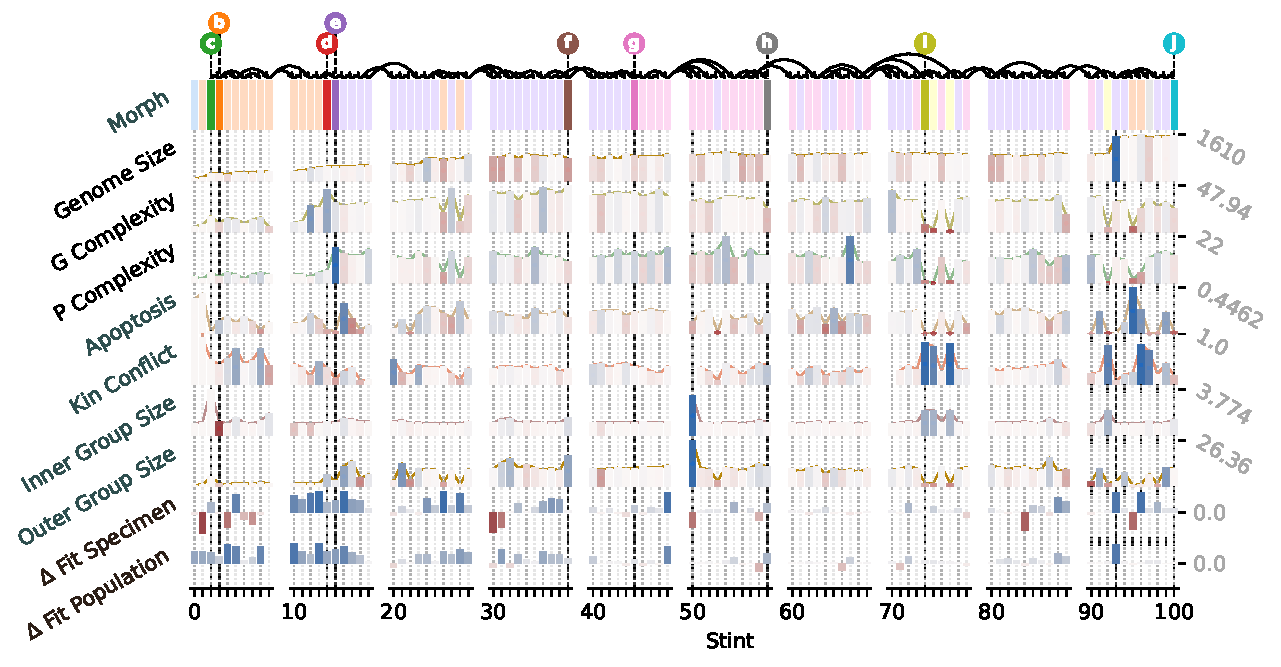
\includegraphics[width=\linewidth]{binder-2025-08-24-keyfig/binder/teeplots/2025-08-24-keyfig/viz=subplots+ext=.pdf}
\caption{%
\textbf{Survey of complexity, novelty, and adaptation across evolutionary history.}
\footnotesize
Columns correspond to 100 specimens sampled at sequential checkpoints across evolutionary history (``stints'').
Top row, ``Morph,'' reports qualitative categorizations of multicell structure for sampled specimens.
Arrows indicate estimated ancestry among specimens.
Bottom rows, ``$\Delta$ Fit Specimen'' and ``$\Delta$ Fit Population'' report results of fitness competitions between current checkpoint and preceding checkpoint.
In specimen assays, sampled specimen from current checkpoint was competed against a whole-population sample from the preceding checkpoint.
In population assays, whole-population sample from current checkpoint was competed against whole-population sample from the preceding checkpoint.
Positive results indicate fitness gain over ``stint,'' while negative results indicate fitness loss.
Middle rows trace evolution of individual traits across sampled specimens.
Color-coding indicates magnitude of change relative to estimated phylogenetic ancestor (blue, positive; red, negative).
G complexity is genetic complexity --- the number of genome sites with detectable fitness effects in knockout experiments.
P complexity is phenotypic complexity --- the number of distinct input/output interfaces between cells and their environment/neighbors that cause fitness loss when disrupted.
Group size is unweighted mean across groups formed in monoculture trials.
}
\end{figure*}
